\documentclass[11pt,a4paper]{article}

\usepackage[margin=0.2in]{geometry}
\usepackage[utf8]{inputenc}
\usepackage[MeX]{polski}
\usepackage{graphicx}
\usepackage{wrapfig}
\usepackage{color}
\usepackage{amsmath}
\usepackage{amssymb}
\usepackage[inkscapelatex=false]{svg}
\usepackage{array, makecell}
\usepackage{mhchem}
\usepackage{tabularx}
\usepackage{braket}
\usepackage{pdfpages}

\usepackage{multicol}
\usepackage{colortbl}
\usepackage[Export]{adjustbox}
\adjustboxset{max size={0.9\linewidth}{0.9\paperheight}}
\usepackage[colorlinks=true,linkcolor=red,citecolor=green]{hyperref}

\textwidth=16cm
\textheight=23cm
\topmargin=-2cm
\oddsidemargin=0cm

\setlength{\parindent}{0em}
\setlength{\parskip}{0.6em}
\setlength{\jot}{12pt}

\renewcommand{\arraystretch}{1.4}
\renewcommand\theadfont{\bfseries}

\newcommand{\todo}[1]{\textcolor{red}{TODO: #1}}

\begin{document}

\title{\textbf{MD - Symulacja Argonu}}
\author{Dawid Karpiński}
\date{23.11.2023 r.}
\maketitle
\pagebreak

\section{Test stabilności programu}

\begin{figure}[ht!]
    \caption{\textbf{Zachowanie symulacji przy różnych krokach czasowych $\tau$}}
    \vspace{0.2cm}
    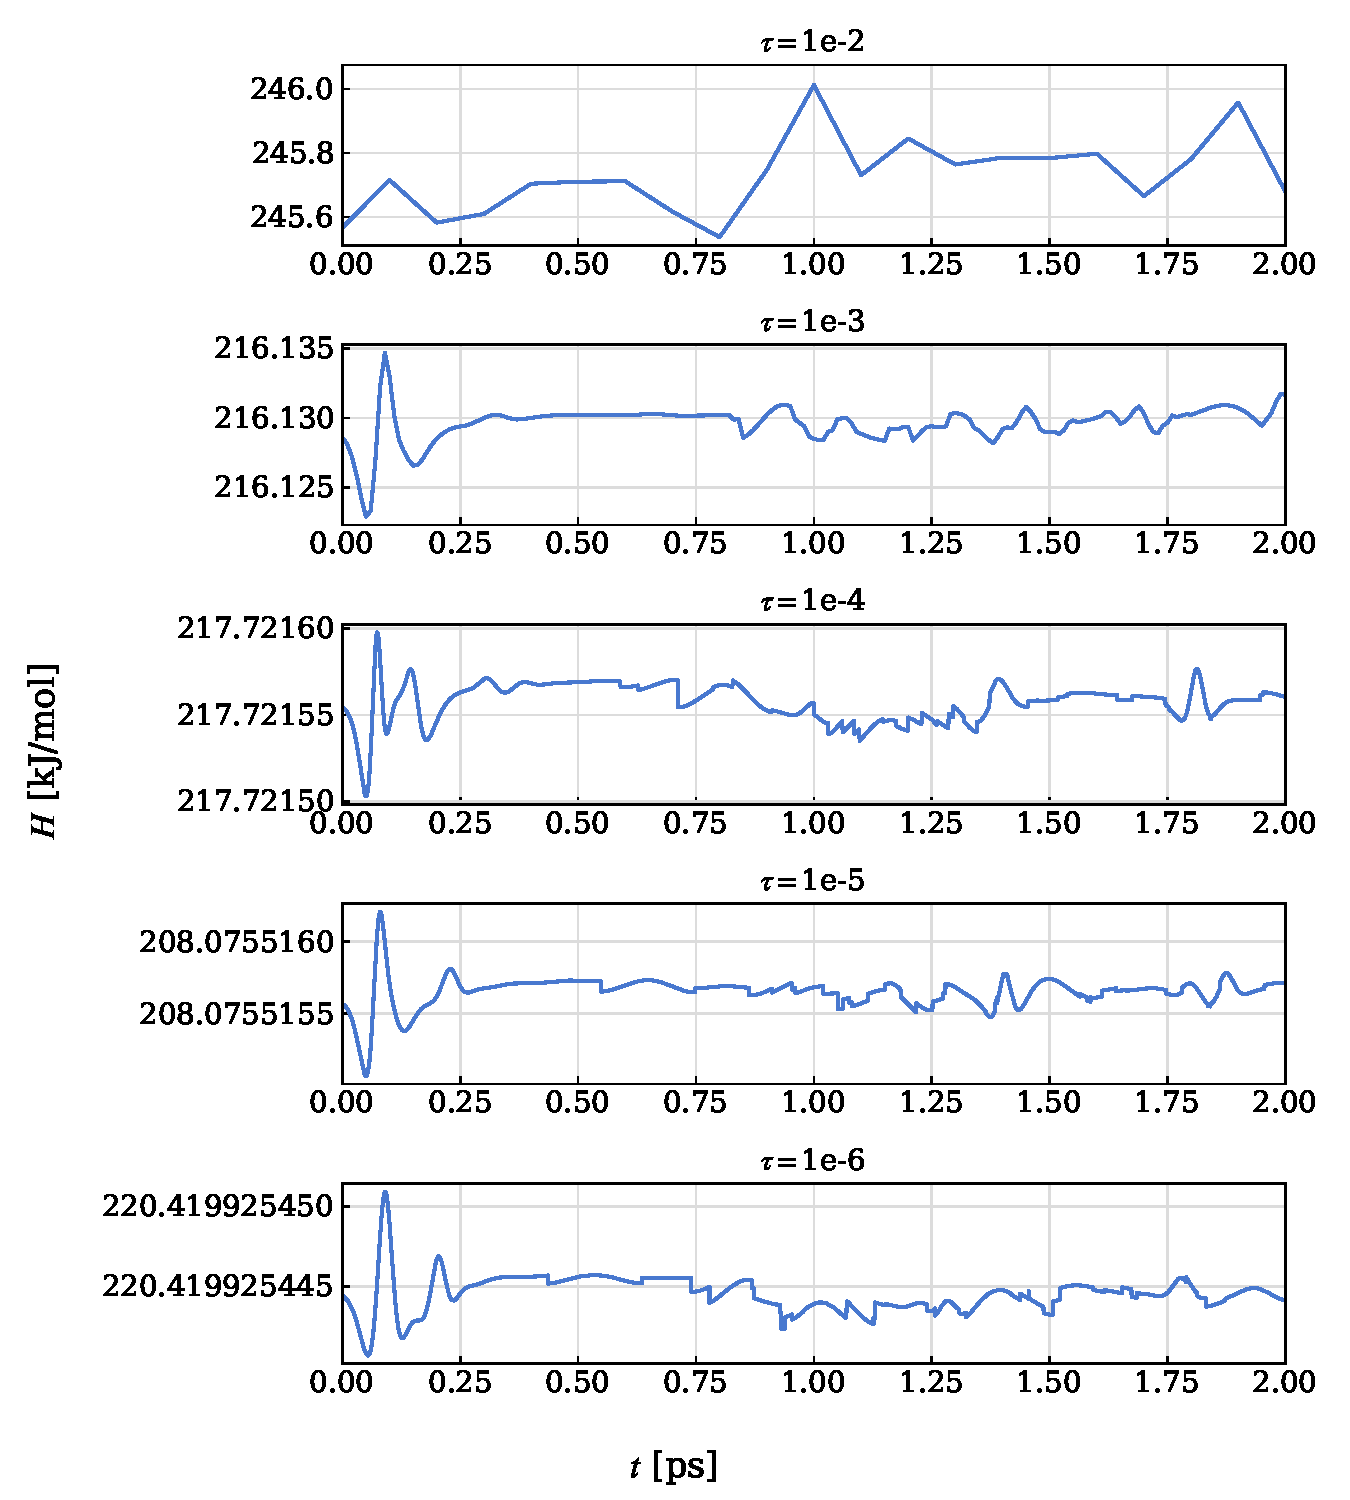
\includegraphics[width=\textwidth]{../figures/stability.pdf}
\end{figure}

Dla zbadanych wartości $\tau$, symulacja wydaje się być stabilna. Przy $\tau=10^{-7}$, zaczynają być widoczne większe fluktuacje w energii. Długi czas wykonywania programu dla mniejszych wartości $\tau$ uniemożliwił dostateczne znalezienie granicy stabilności.

\section{Kryształ}

Najniższą energię potencjalną otrzymano dla wartości $a\approx0.37$ [nm].

\begin{figure}[ht!]
    \caption{\textbf{Zależność energii potencjalnej $V$ od wartości $a$}}
    \vspace{0.2cm}
    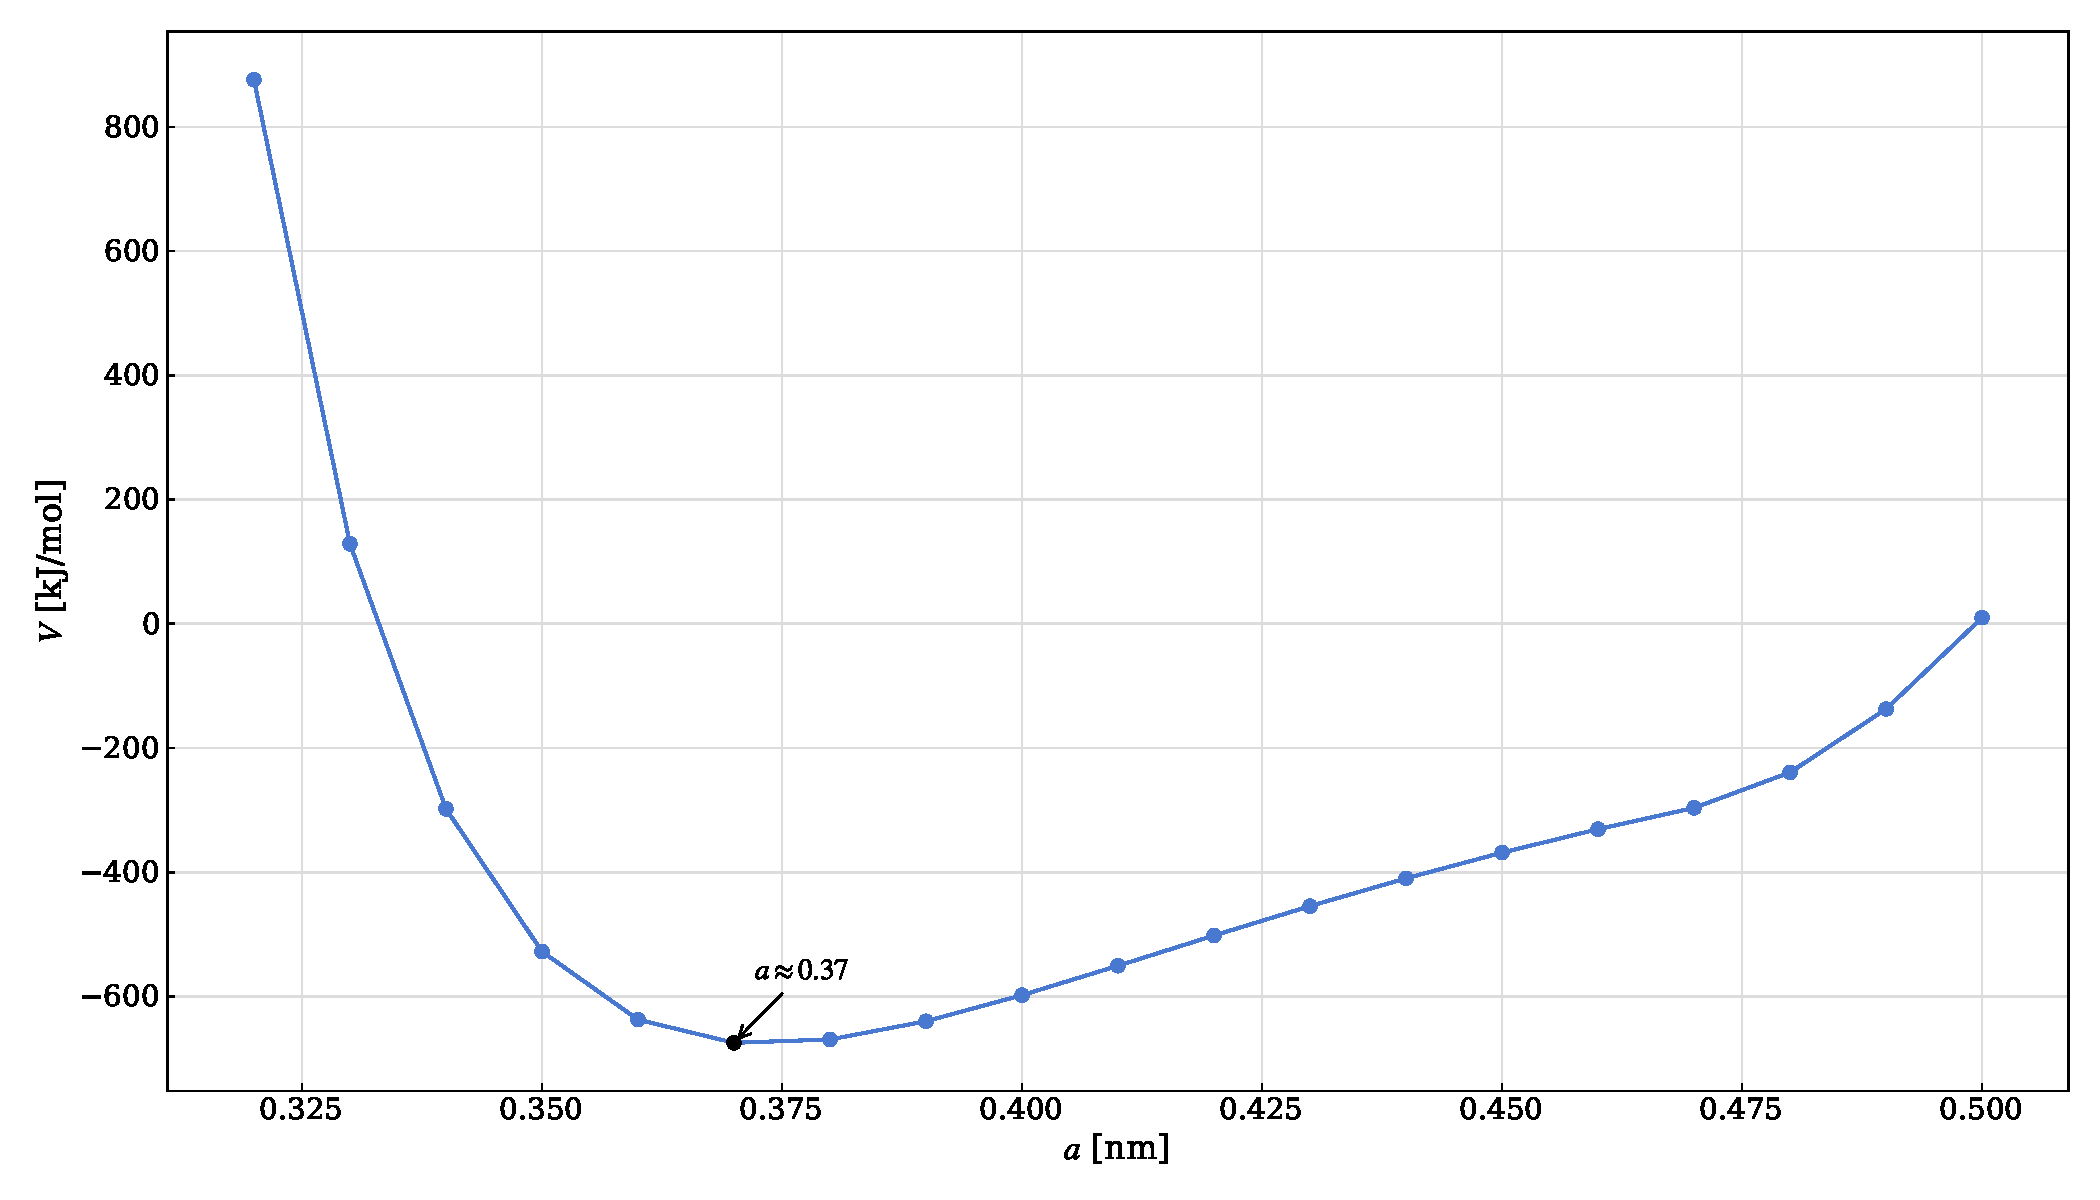
\includegraphics[width=\textwidth]{../figures/plot_V_vs_a.pdf}
\end{figure}

Średnia temperatura po czasie 1 [ps] wyniosła: $T_{\text{avg}}\approx0.6925$ [K] $>$ 0 [K]. Dzieje się tak, ze względu na ograniczenia numeryczne liczb zmienno przecinkowych w pamięci komputera. Według mechaniki kwantowej, najmniejsza energia jest zwykle większa od zera, dlatego kryształ może ustalić się na temperaturze większej niż 0 [K] (przez tzw. drgania zerowe).

W praktyce natomiast, jest to wynik ograniczeń numerycznych pamięci komputera i aproksymacji użytych w symulacji. Nie jest zatem możliwe dokładne odwzorowanie stanu o zerowej energii kinetycznej. Układ więc ustala się na niskiej, ale niezerowej temperaturze.

Warto zauważyć, że temperatura 0K, znana jako zero bezwzględne, jest teoretyczną granicą, do której można ochłodzić układ termodynamiczny1. W rzeczywistości, osiągnięcie temperatury 0K jest niemożliwe z powodu trzeciej zasady termodynamiki1.

\begin{figure}[ht!]
    \caption{\textbf{Zależność hamiltonianu $H$ od czasu $t$ kryształu o znalezionej stałej sieci}}
    \vspace{0.2cm}
    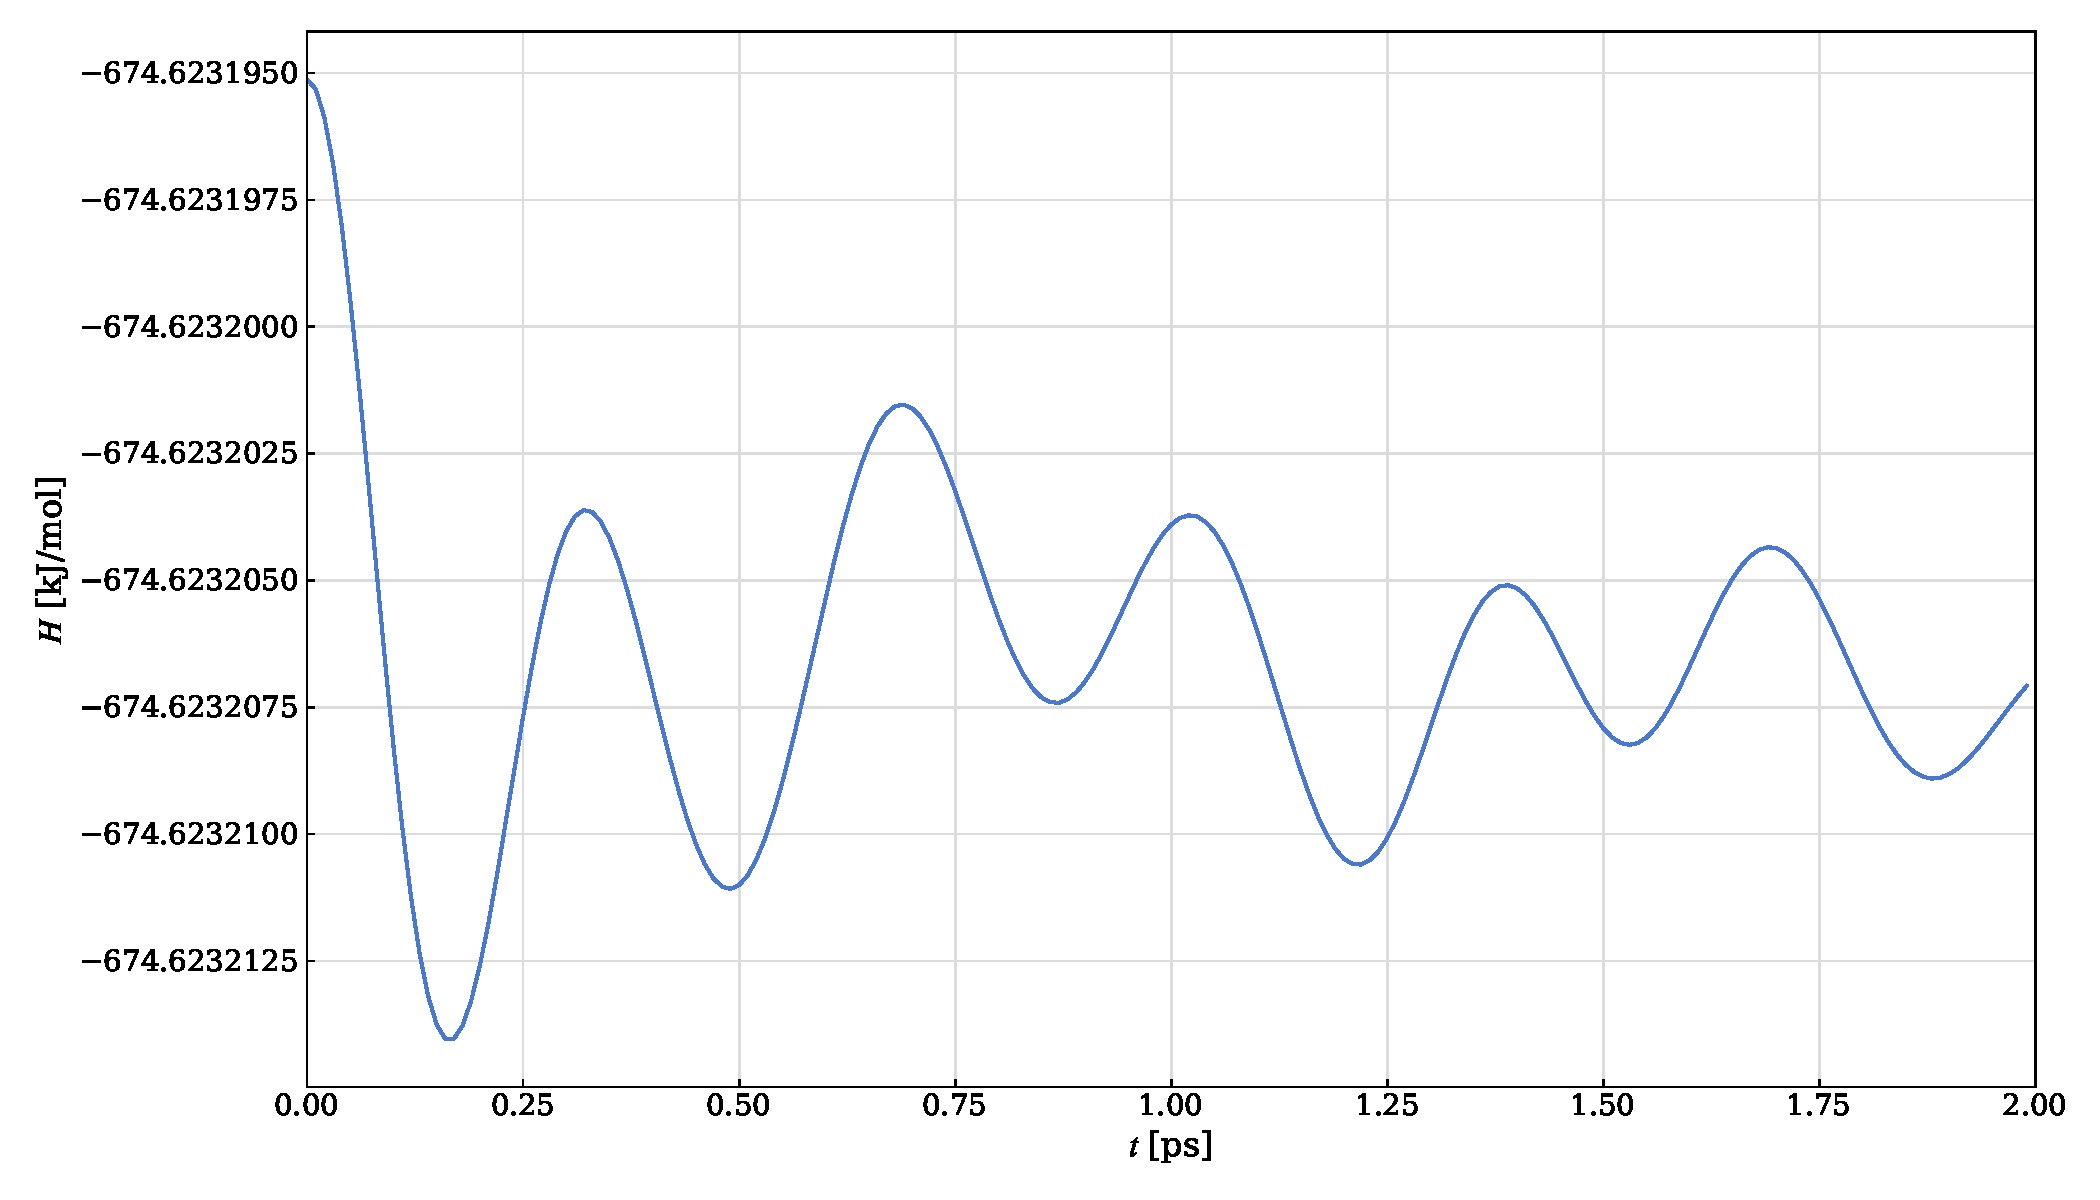
\includegraphics[width=\textwidth]{../figures/crystal_stability.pdf}
\end{figure}
\pagebreak

 Wartość hamiltonianu zmienia się dopiero na czwartym miejscu po przecinku, co świadczy o niewielkiej fluktuacji.

\subsection{Topnienie kryształu}

\begin{figure}[ht!]
\caption{\textbf{Zachowanie kryształu w: $T=10$ [K], $T=70$ [K], $T=130$ [K]}}
\begin{multicols}{3}
    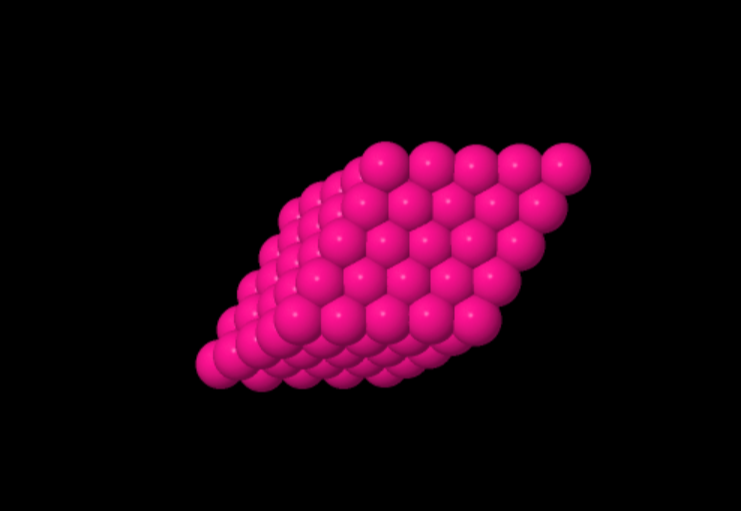
\includegraphics[width=\linewidth]{../figures/crystal.png}
    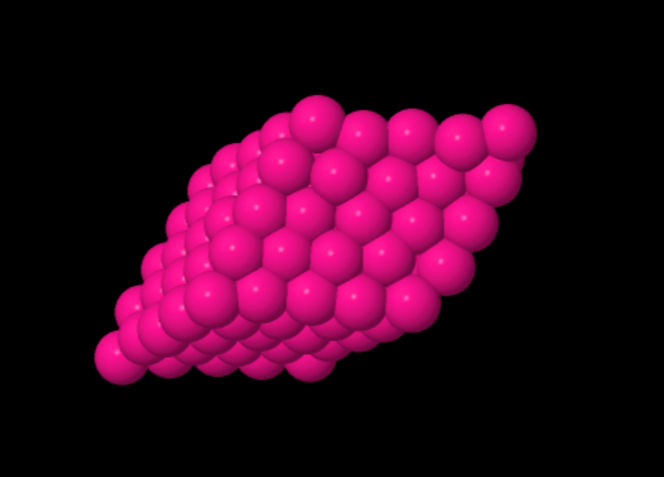
\includegraphics[width=\linewidth]{../figures/melting.png}
    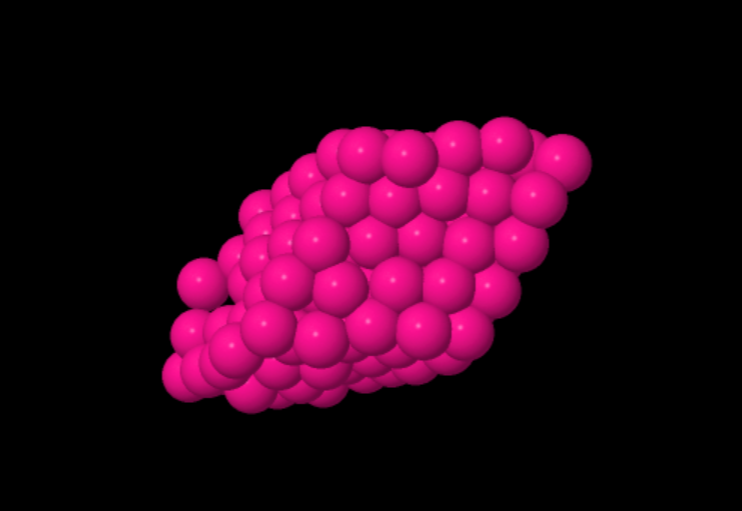
\includegraphics[width=\linewidth]{../figures/melted.png}
\end{multicols}
\end{figure}

Temperaturę topnienia oszacowano na około $T=70$ [K], ponieważ struktura regularna kryształu zaczyna się widocznie załamywać w granicach 60 - 80 [K].

\section{Gaz}

\subsection{Porównanie z gazem doskonałym}
Na koniec, porównano zależność ciśnienia od temperatury z danych symulacji do zależności teoretycznej:

$$
P(T) = \frac{3}{2} \frac{N k_B T}{V}
$$

\begin{figure}[ht!]
    \caption{\textbf{Porównanie zależności P(T) dla danych pomiarowych i gazu doskonałego}}
    \vspace{0.2cm}
    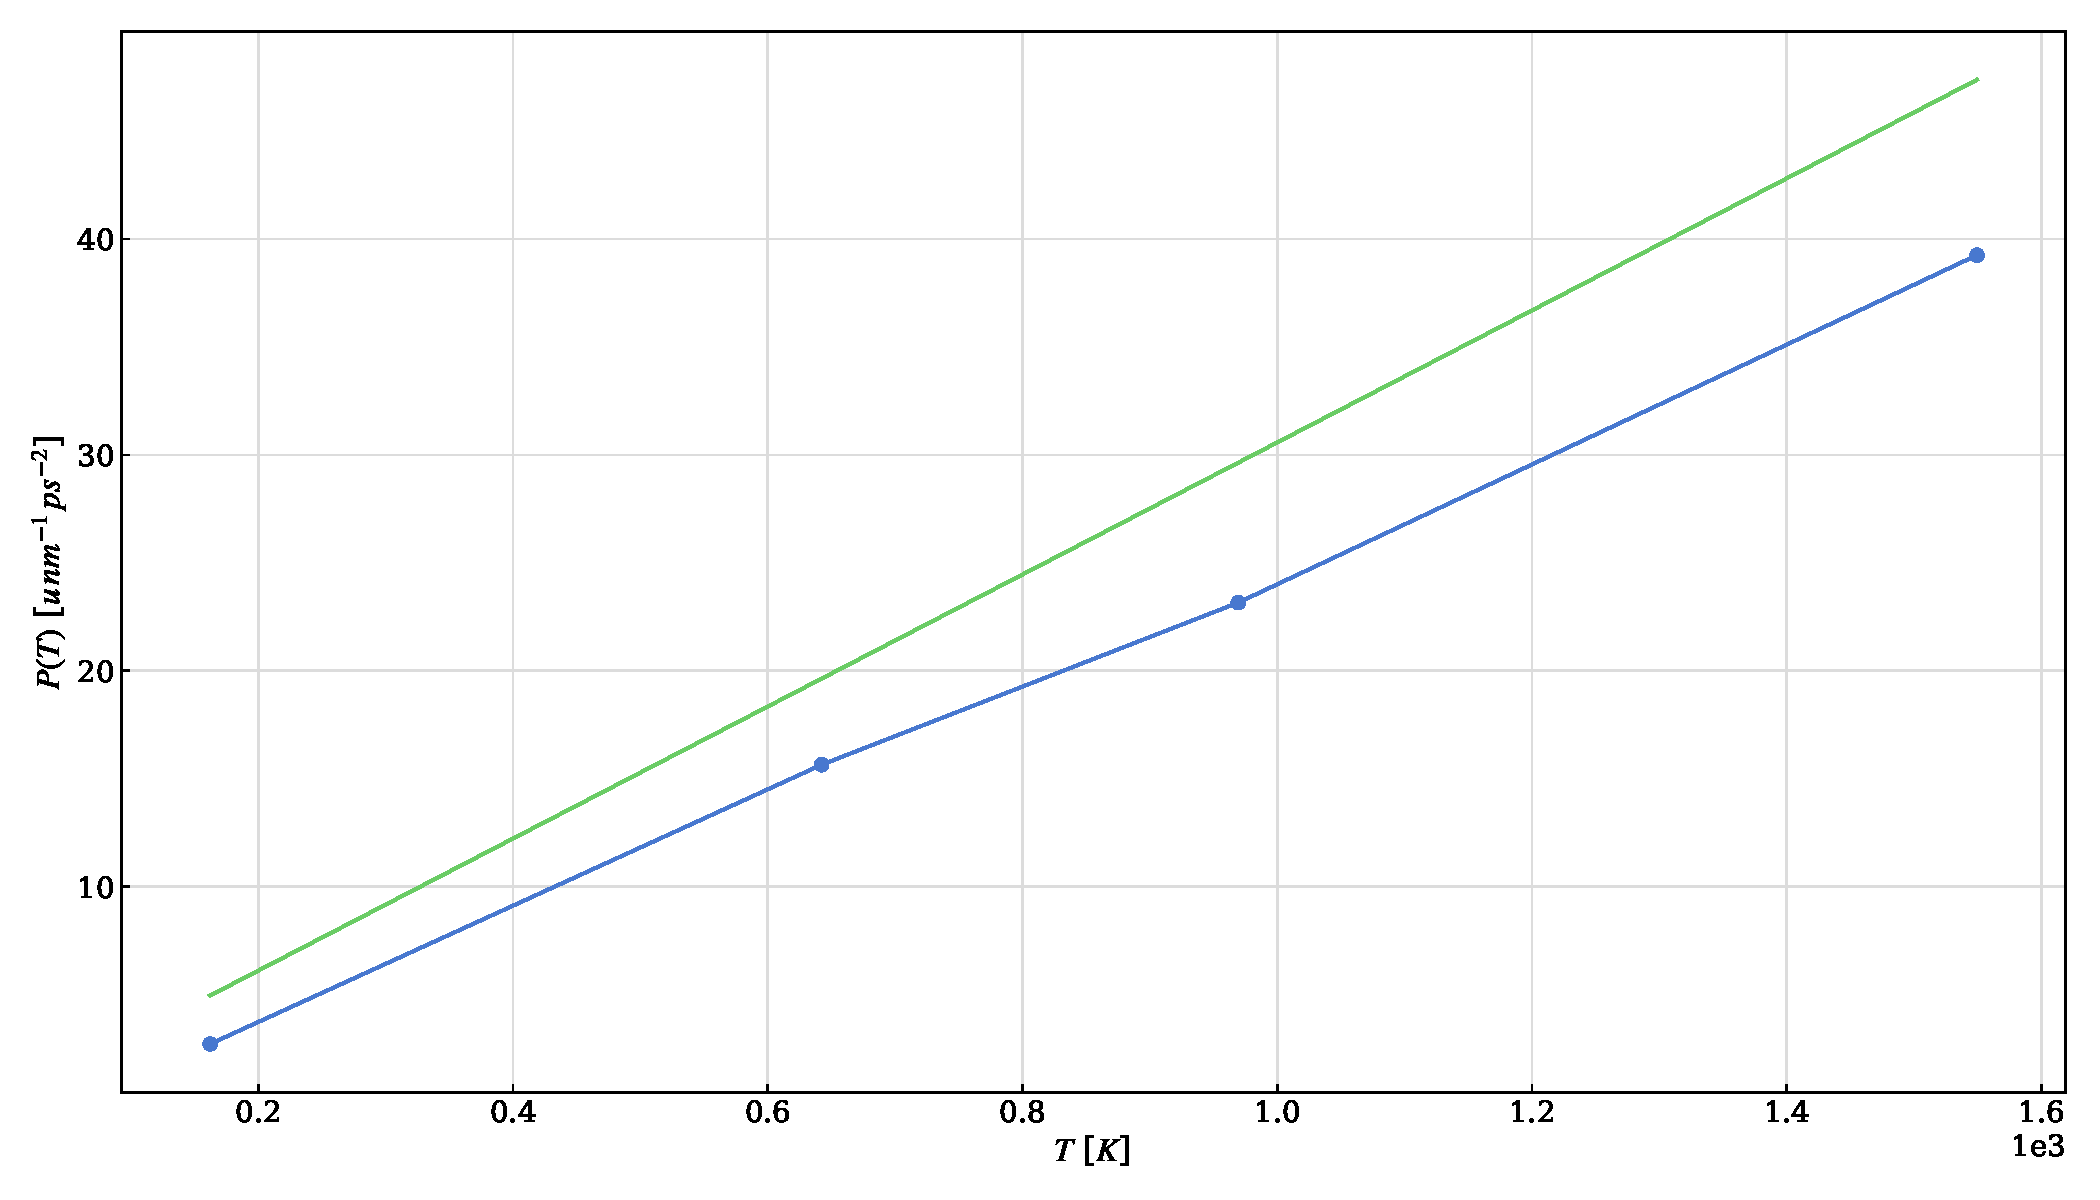
\includegraphics[width=\textwidth]{../figures/P_vs_T.pdf}
\end{figure}

Na koniec przedstawiono wykresy: Hamiltonian od czasu i ciśnienie od czasu dla każdego z powyżych punktów:

\begin{figure}[ht!]
    \caption{\textbf{Zestawienie zależności $H(T)$ i $P(T)$ dla badanych czterech punktów}}
    \vspace{0.2cm}
    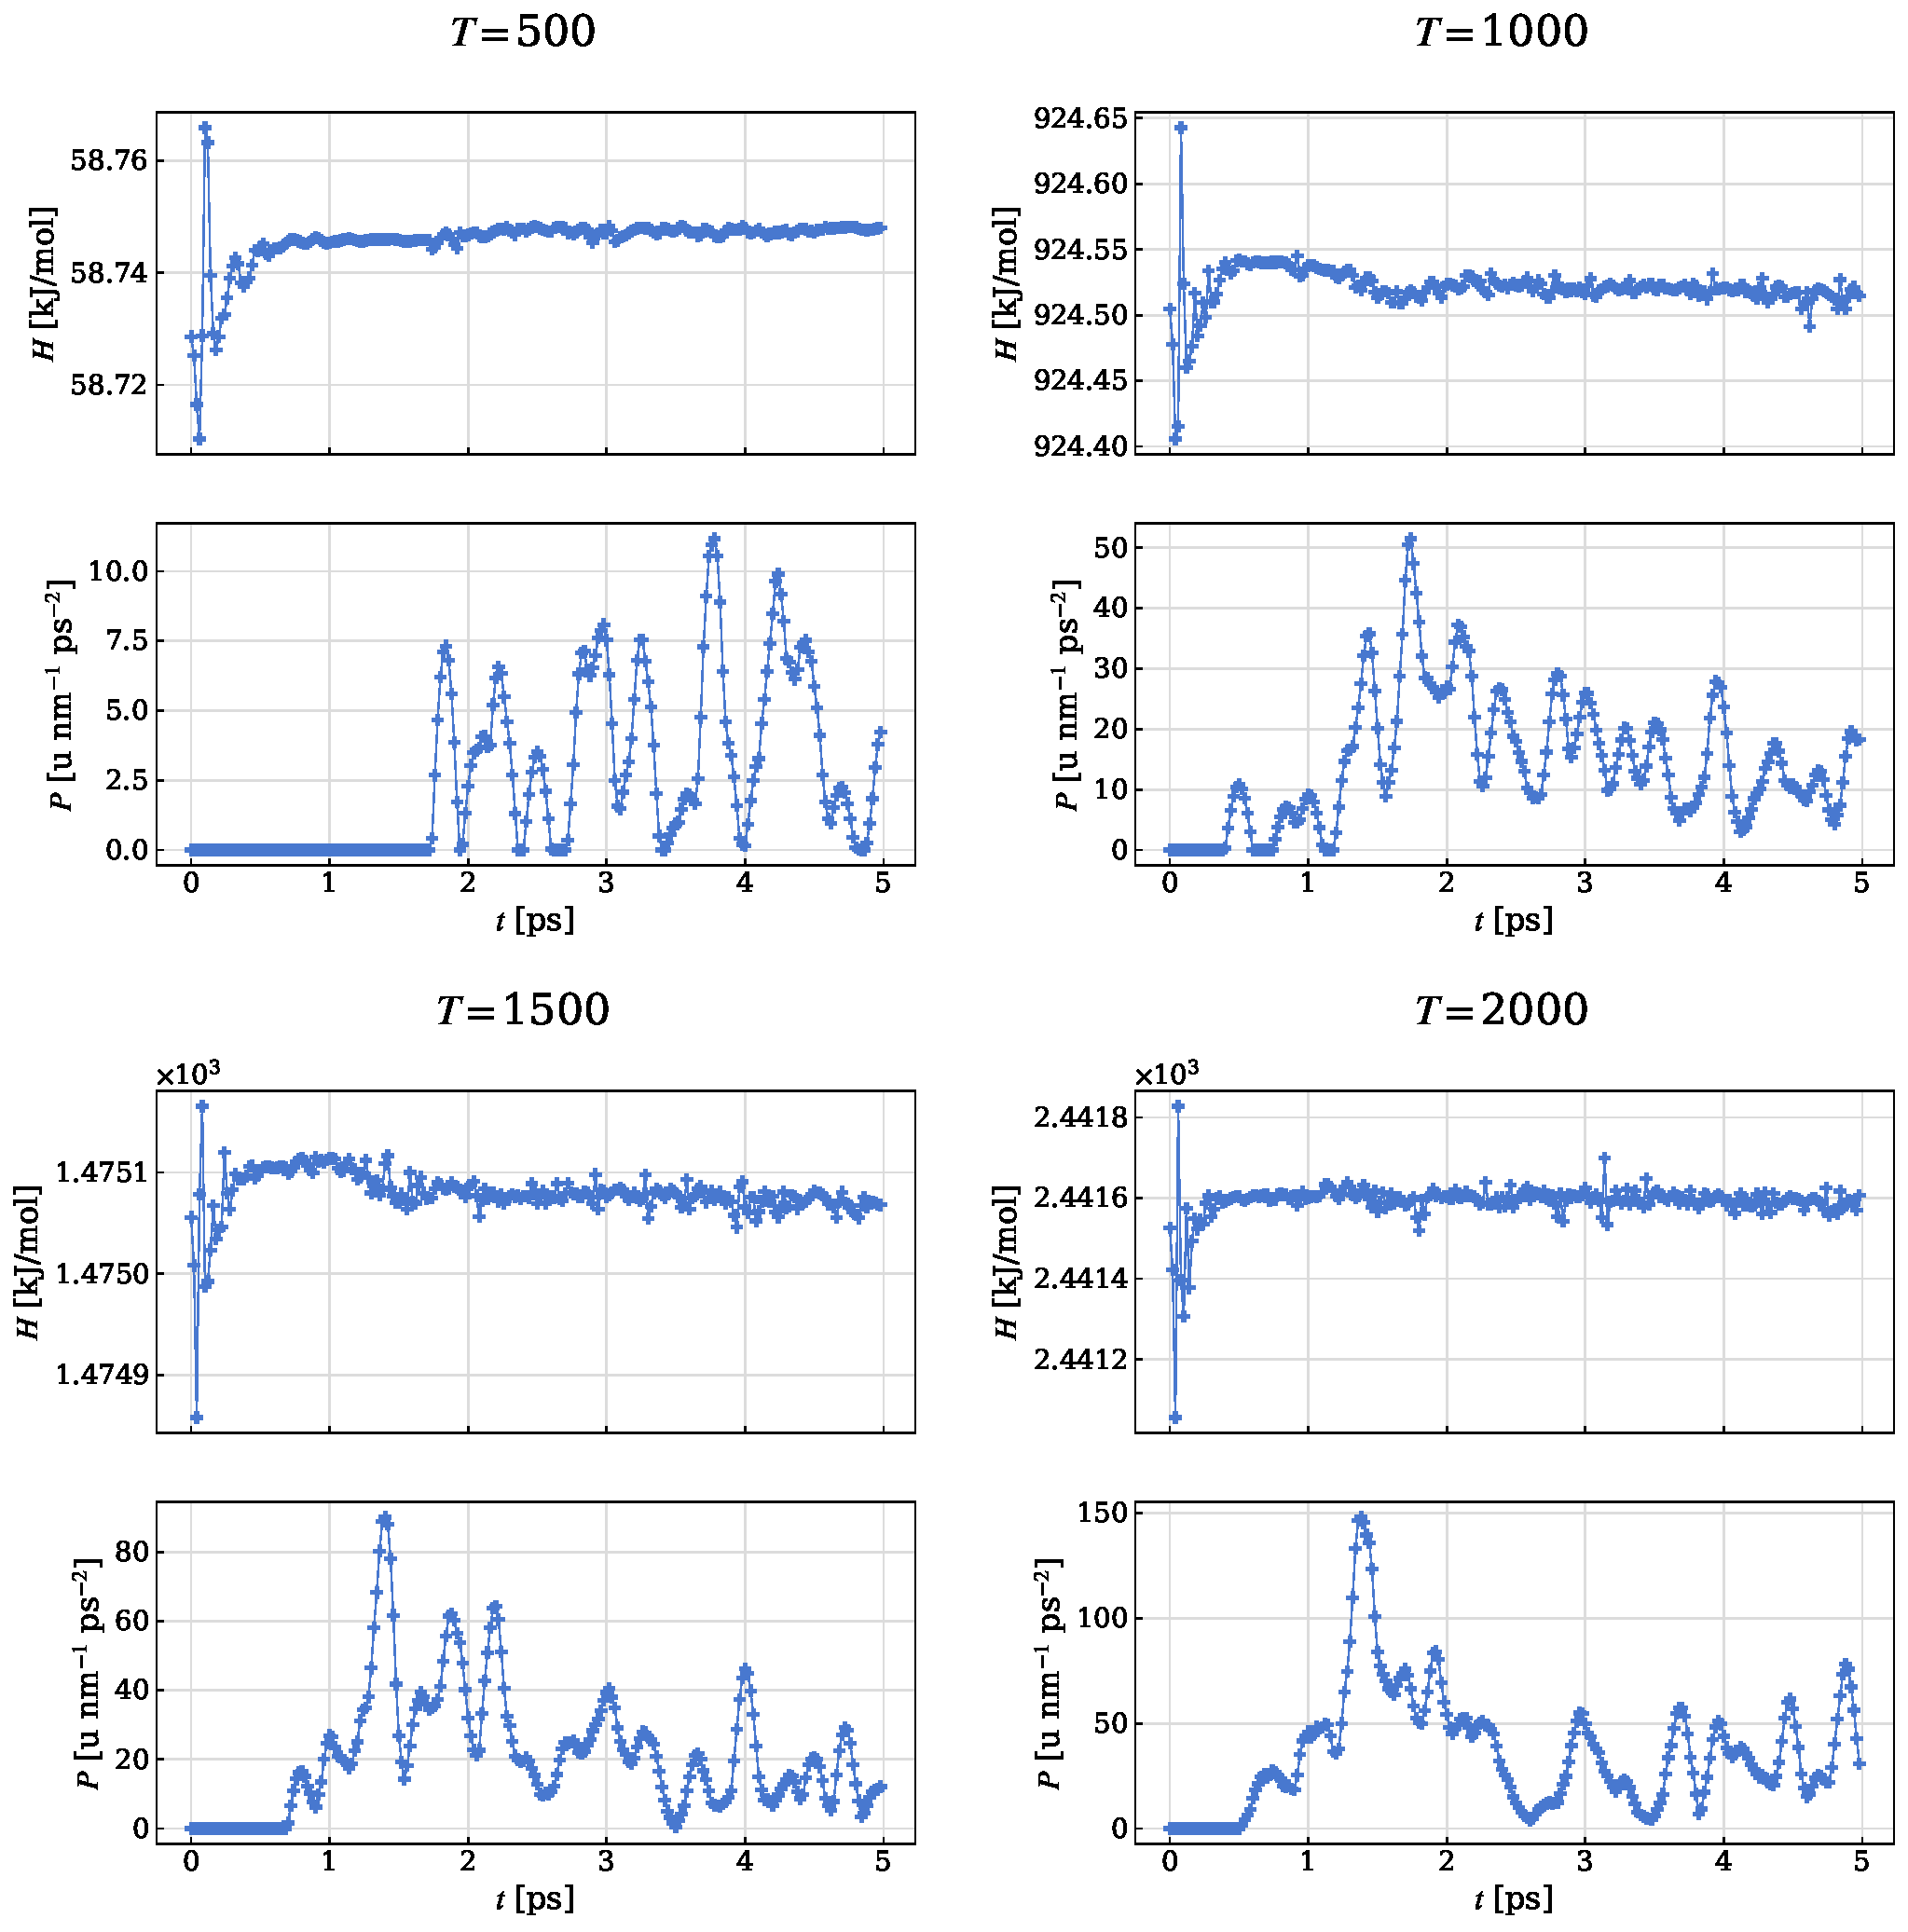
\includegraphics[width=\linewidth]{../figures/gas_stability.pdf}
\end{figure}
\pagebreak

\section{Podsumowanie}

Kod programu oraz wszelkich skryptów do zbierania i analizy danych znajduje się w repozytorium: \url{https://github.com/davkk/argon-simulation}.

Do wykonania zadania wykorzystałem takie technologie i narzędzia jak: Python (Numba), Bash (GNU Parallel, awk, itd.), JMOL.

\end{document}
